\chapter{Software}

\section{Communication Core}
Paul -done

\section{CarControl Core}
Johannes / code kommentieren

\section{Shared memory Controller}
Johannes / code kommentieren

\section{Motor Controller}
Johannes / code kommentieren

\section{CarProtocol}
It was part of the work of the previous lab-course group to set up a communication protocol for the car. As the communication was realized using telnet streams, they decided to add another layer over the already existing TCP/IP and telnet protocol layer. This means that the actual protocol for the car is represented by the payload of telnet messages, representing just characters.
\\ \\
In fact, the actual message must be parsed from the incoming telnet  characters. Therefore the so called \glqq CARP\grqq \ or \glqq Car-Protocol\grqq \ consists of packets and messages. Every packet consists of a CARP header and several CARP messages what makes it possible to search the incoming telnet stream for the CARP header and extract all the reqired information about the messages which are part of the specific packet.
\\ \\
For giving a rough idea on how this structure is assembled, here is a figure from Florian Hisch, showing the header-packet-message setup. For a more detailed description have a look at chapter 4.3 of the WS13/14 groups documentation.

\begin{figure}[ht]
	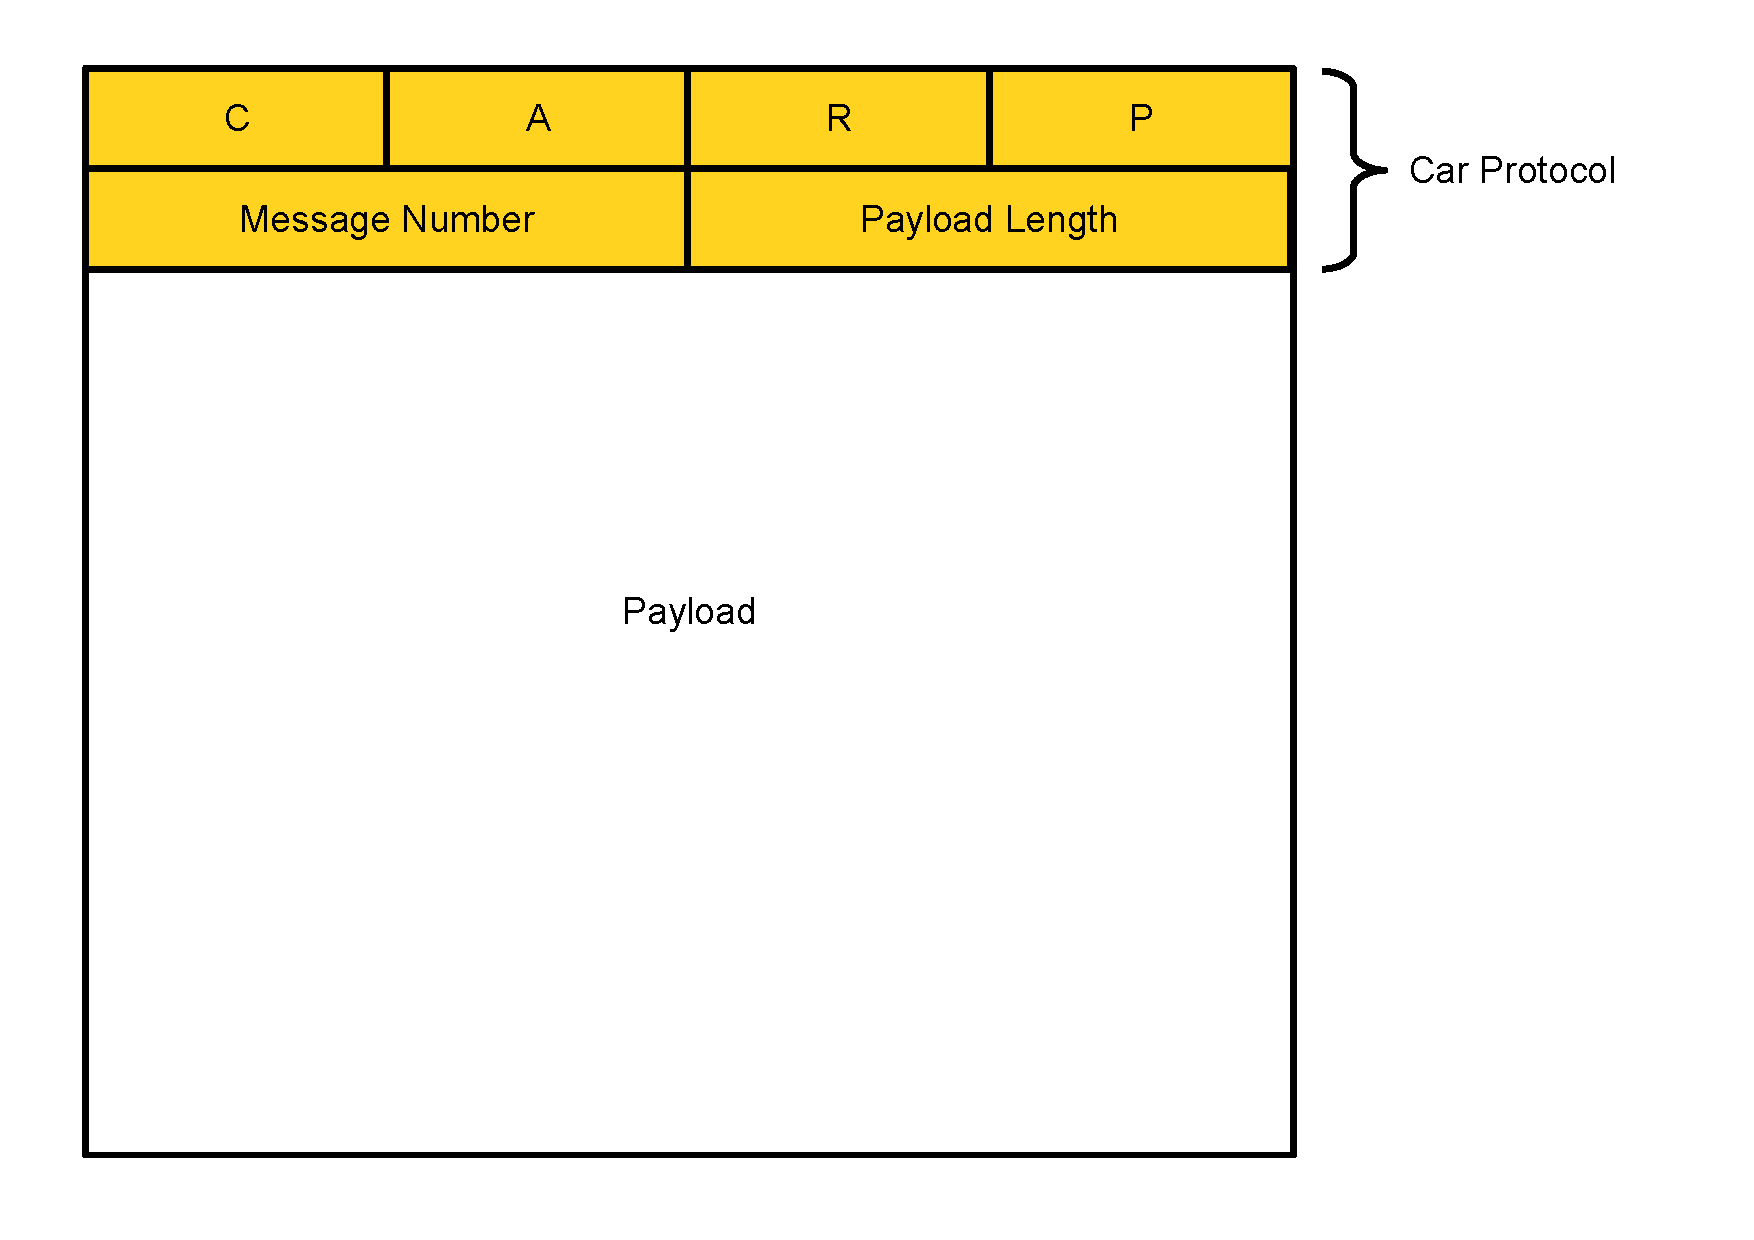
\includegraphics[width=0.5\textwidth]{figures/prot0.pdf}
	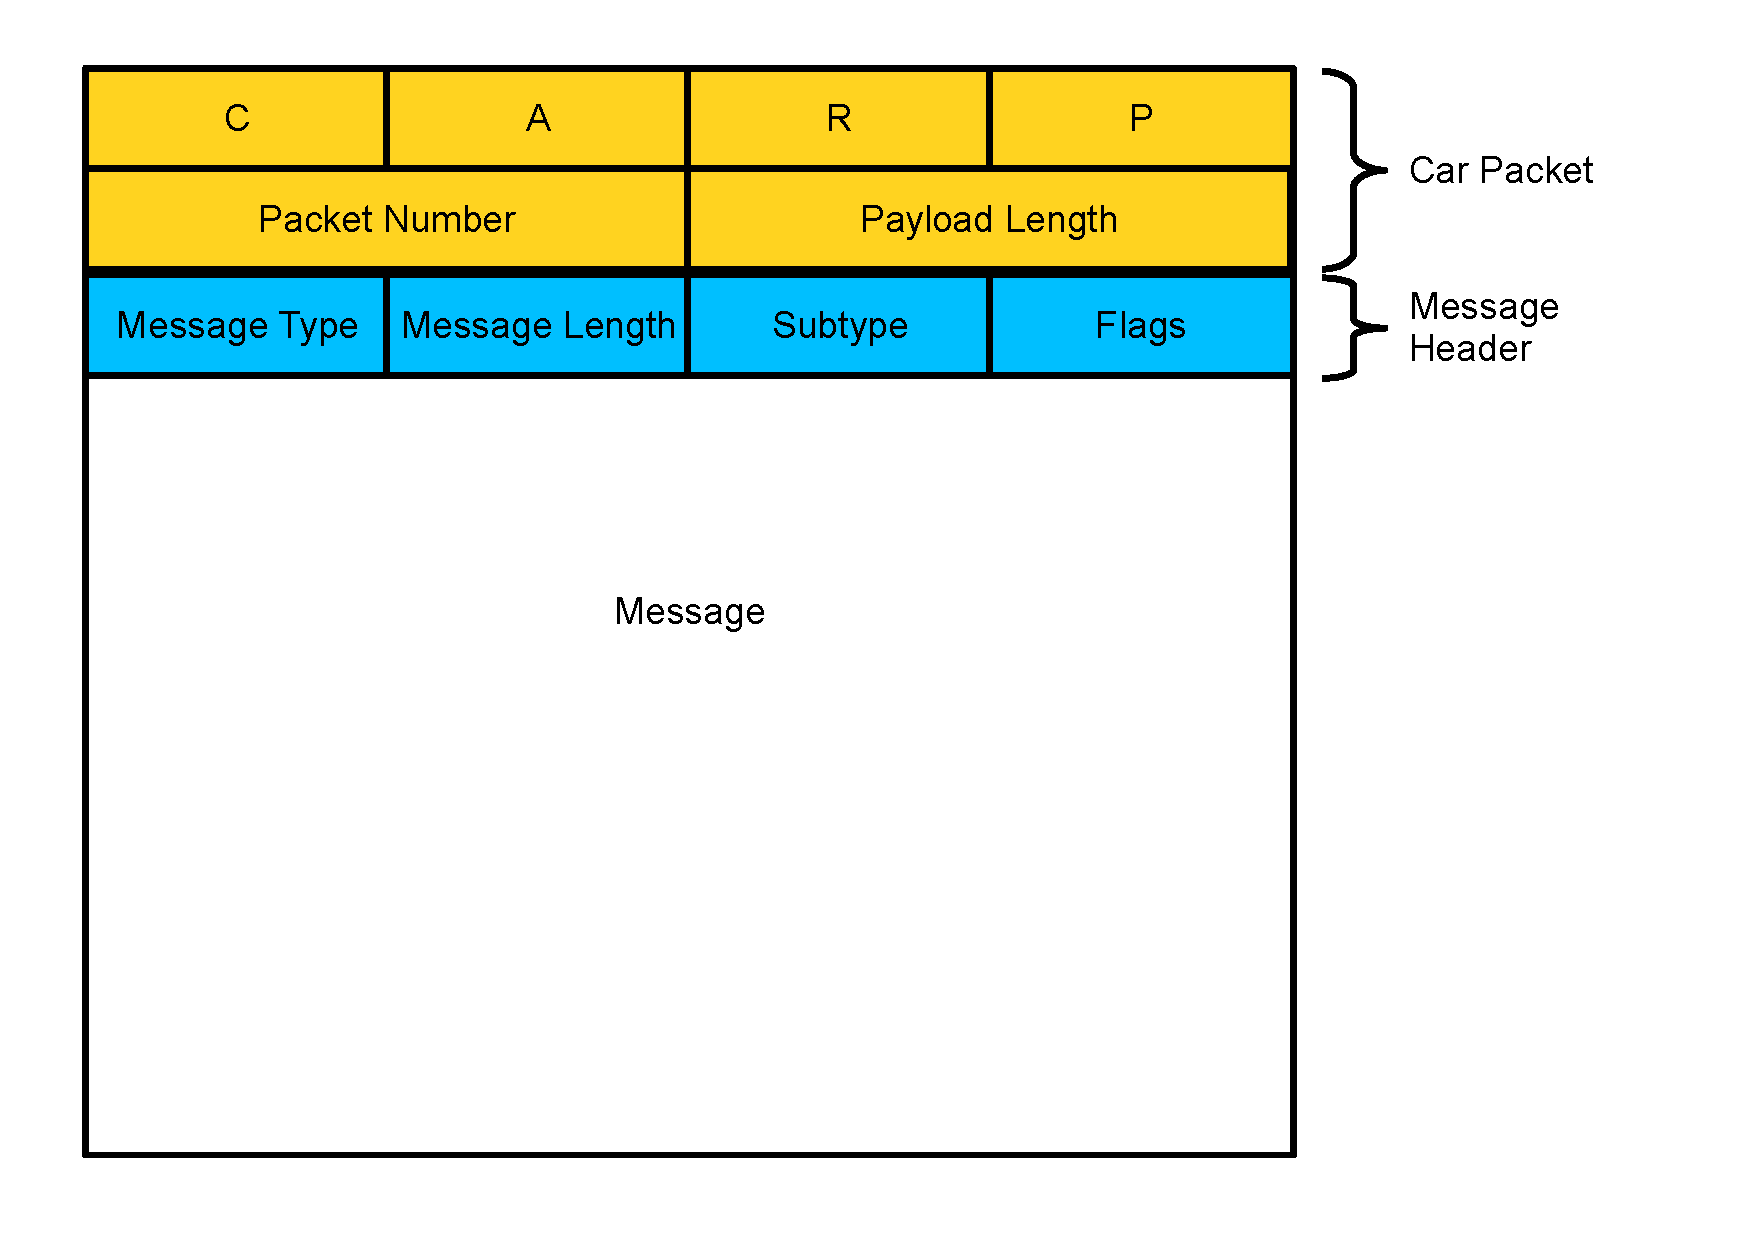
\includegraphics[width=0.5\textwidth]{figures/prot1.pdf}
	\caption{Left: CarProtocol header. Right: CarMessage header.} \label{CarProtocol}
\end{figure}

\section{C2X extensions}
There are basically two types of CAR2X messages. \glqq Polling messages\grqq \ and \glqq Triggering messages\grqq \ which have nearly the same structure as CARP messages. The only difference is that these messages are intended to establish communication with clients other than the core-car-parts. To make it easy to identify CAR2X messages, their 8 bit type-value always has the 4 least significant bits equal to zero: 0xV0  with $0x1\leq V\leq 0xF$.\\ \\
In case of simple \glqq Polling messages\grqq \ that don’t interact with the car state, like the \glqq CInfoStateMessage\grqq \ and the \glqq CInfoSensorMessage\grqq \ which do only read some information out of the current state, there is immediately created and sent an answer message, containing the required data, after the message is executed by the car.\\
The other three messages have an influence on the car state and therefore have to be queued until the car state gets updated. Once the update is there, the main loop of the socketserver checks if the requested state change like for example an emergency brake process has been performed or not, deletes the message from the queue and sends an answer message. Depending on this check the produced answer message contains a different flag: 
\begin{itemize}
\item \glqq A\grqq \ for successful execution(\glqq Answer\grqq)
\item \glqq F\grqq \ for failed execution
\item \glqq O\grqq \ for the message being outdated
\end{itemize}
The main challenge and reason for this check is the fact that communication and state control are performed by different NIOS2 cores. While the state is being updated periodically, incoming messages might arrive more frequent. If for example 3 \glqq CControlMessages\grqq , which contain the information to set the motors to a specific speed, are received within one state update cycle, it is obvious that only the last one should be executed in the new state and the older ones get outdated as soon as a new message of the same type is received. Whenever a message gets queued, and there is already a message in the queue, the outdated one gets immediately answered with an \glqq O\grqq \ flag. This message then is outdated and doesn’t have to be executed any more, since it has been overwritten by the latest message, resulting in only one queued message at maximum for every message type at every state update. For more information about the queueing process read the Communication Core chapter.\\ \\
In the following part all types of CAR2X messages are xplained using examples. Note that there is always the protocol header included.
For answer messages the protocol header consists of CARP, \glqq ControlCoreCounter\grqq ,\glqq CommCoreCounter\grqq \, payloadLength, success-flag and message type.

\subsection*{CEmergencyBrakeMessage}
Example packet sent to the car:\\
\resizebox{\linewidth}{!}{
\renewcommand{\arraystretch}{1.5}
\begin{tabular}{|c||c|c|c|c|c|c|c|c|c|c|}
\hline 
\rule[-1ex]{0pt}{2.5ex} Byte & 1 & 2 & 3 & 4 & 5 + 6 & 7 + 8 & 9 & 10 & 11 & 12 \\ 
\hline 
\rule[-1ex]{0pt}{2.5ex} Inhalt & C & A & R & P & PacketID & PayloadLength: 0x04 & Type: 0x20 & Length: 0x04 & Subtype: 0x0 & Flags: 0x0 \\ 
\hline 
\end{tabular}} \\
\newline
\newline
After receiving this message, the control core is requested to change the car state into emergency braking and this message is queued to wait for the next state update, or being outdated.\\
\newline
The payload of the answer consists of the PacketNumber of the received message.\\
\newline
Example answer message sent by the car:\\
\resizebox{\linewidth}{!}{
\renewcommand{\arraystretch}{1.5}
\begin{tabular}{|c||c|c|c|c|c|c|c|c|c|c|}
\hline 
\rule[-1ex]{0pt}{2.5ex} Byte & 1 & 2 & 3 & 4 & 5 - 8 & 9 - 12 & 13 - 16 & 17 & 18 & 19 + 20 \\ 
\hline 
\rule[-1ex]{0pt}{2.5ex} Inhalt & C & A & R & P & ControlCoreCounter & CommCoreCounter & PayloadLength & Success flag (‘A’,’F’,’O’) & Type: 0x20 & PacketID of the received message \\ 
\hline 
\end{tabular}}

\subsection*{CControlMessage}
Example packet sent to the car:\\
\resizebox{\linewidth}{!}{
\renewcommand{\arraystretch}{1.5}
\begin{tabular}{|c||c|c|c|c|c|c|c|c|c|c|c|c|c|c|}
\hline 
\rule[-1ex]{0pt}{2.5ex} Byte & 1 & 2 & 3 & 4 & 5 + 6 & 7 + 8 & 9 & 10 & 11 & 12 & 13 + 14 & 15 + 16 & 17 + 18 & 19 + 20 \\ 
\hline 
\rule[-1ex]{0pt}{2.5ex} Inhalt & C & A & R & P & PacketID & PayloadLength: 0x0C & Type: 0x30 & Length: 0x0C & Subtype: 0x0 & Flags: 0x0 & V1 & V2 & V3 & V4 \\ 
\hline 
\end{tabular}} \\
\newline
\newline
After receiving this message, the control core is requested to set the specified motor velocities (V1...4 as 16-bit values), specified in the payload. It has to be mentioned that in case the sender of this message is not registered as the current source of control, the message is not queued but immediately replied as failed because the sender is not allowed to control the car.
But if the control is allowed, this message is queued to wait for the next state update, or getting out of date.\\
\newline
Example answer message sent by the car:\\
\resizebox{\linewidth}{!}{
\renewcommand{\arraystretch}{1.5}
\begin{tabular}{|c||c|c|c|c|c|c|c|c|c|c|c|c|c|c|}
\hline 
\rule[-1ex]{0pt}{2.5ex} Byte & 1 & 2 & 3 & 4 & 5 - 8 & 9 - 12 & 13 - 16 & 17 & 18 & 19 + 20 & 21 + 22 & 23 + 24 & 25 + 26 & 17 + 28\\ 
\hline 
\rule[-1ex]{0pt}{2.5ex} Inhalt & C & A & R & P & ControlCoreCounter & CommCoreCounter & PayloadLength & Success flag (‘A’,’F’,’O’) & Type: 0x30 & PacketID of the received message & V1 & V2 & V3 & V4\\ 
\hline 
\end{tabular}}\\
\newline
V1 to V4 are now standing for the current desired motor speed values delivered to the specific PWM motor controllers. In case of a successful message, they are equal to the requested values of the message, sent to the car, otherwise they differ and the message is answered as \glqq failed\grqq , giving the controlling unit feedback about the current state of the car, to let it know what might have failed.

\subsection*{CRemoteControlMessage}
Example packet sent to the car:\\
\resizebox{\linewidth}{!}{
\renewcommand{\arraystretch}{1.5}
\begin{tabular}{|c||c|c|c|c|c|c|c|c|c|c|c|c|c|c|}
\hline 
\rule[-1ex]{0pt}{2.5ex} Byte & 1 & 2 & 3 & 4 & 5 + 6 & 7 + 8 & 9 & 10 & 11 & 12 & 13 & 14 & 15 & 16 \\ 
\hline 
\rule[-1ex]{0pt}{2.5ex} Inhalt & C & A & R & P & PacketID & PayloadLength: 0x08 & Type: 0x60 & Length: 0x08 & Subtype: 0x0 & Flags: 0x0 & IP1 & IP2 & IP3 & IP4 \\ 
\hline 
\end{tabular}} \\
\newline
\newline
The payload of this message contains the IP of a source which should be allowed to control the car by using \glqq CControlMessages\grqq . Per default this source is the unit inside of the car featuring the ImageProcessingUnit with its IP 192.168.0.110. In the standard state of the car \glqq AutoDrive\grqq , the car is controlled from this IP by \glqq CControlMessages\grqq . By sending a \glqq CRemoteControlMessage\grqq \ to the car containing a different IP, the car is requested to set its state to \glqq ManualDrive\grqq \ with the new source IP locked for \glqq CControlMessages\grqq . Sending 0.0.0.0 as new IP will set the car back to \glqq AutoDrive\grqq , using the ImageProcessing IP again.
As before, the answer gets queued until the state is updated for the next time.\\
\newline
Example answer message sent by the car:\\
\resizebox{\linewidth}{!}{
\renewcommand{\arraystretch}{1.5}
\begin{tabular}{|c||c|c|c|c|c|c|c|c|c|c|c|c|c|c|}
\hline 
\rule[-1ex]{0pt}{2.5ex} Byte & 1 & 2 & 3 & 4 & 5 - 8 & 9 - 12 & 13 - 16 & 17 & 18 & 19 + 20 & 21 + 22 & 23 + 24 & 25 + 26 & 17 + 28\\ 
\hline 
\rule[-1ex]{0pt}{2.5ex} Inhalt & C & A & R & P & ControlCoreCounter & CommCoreCounter & PayloadLength & Success flag (‘A’,’F’,’O’) & Type: 0x60 & PacketID of the received message & IP1 & IP2 & IP3 & IP4\\ 
\hline 
\end{tabular}}\\
\newline
IP1 to IP4 are the current state values of the locked IP. In case of success they equal the requested one, otherwise they give the feedback about who is currently controlling the car.

\subsection*{CInfoStateMessage}
Example packet sent to the car:\\
\resizebox{\linewidth}{!}{
\renewcommand{\arraystretch}{1.5}
\begin{tabular}{|c||c|c|c|c|c|c|c|c|c|c|c|c|c|c|}
\hline 
\rule[-1ex]{0pt}{2.5ex} Byte & 1 & 2 & 3 & 4 & 5 + 6 & 7 + 8 & 9 & 10 & 11 & 12 & 13 & 14 & 15 & 16 \\ 
\hline 
\rule[-1ex]{0pt}{2.5ex} Inhalt & C & A & R & P & PacketID & PayloadLength: 0x04 & Type: 0x40 & Length: 0x04 & Subtype: 0x0 & Flags: 0x0\\ 
\hline 
\end{tabular}} \\
\newline
\newline
This message just polls the current state information from the car. It is answered immediately and thus has not to be queued. The answer always contains the \glqq A\grqq \ flag for success and features the biggest part of the state object from the shared memory as its payload. It can be used for debugging purposes or by the ImageProcessing unit or a station as additional odometry feedback\\
\newline
Example answer message sent by the car:\\
\resizebox{\linewidth}{!}{
\renewcommand{\arraystretch}{1.5}
\begin{tabular}{|c||c|c|c|c|c|c|c|c|c|c|c|c|c|c|c|c|c|c|c|c|c|c|c|c|c|c|}
\hline 
\rule[-1ex]{0pt}{2.5ex} Byte & 1 & 2 & 3 & 4 & 5 - 8 & 9 - 12 & 13 - 16 & 17 & 18 & 19 + 20 & 21 - 24 & 25 & 26 & 27 & 28 & 29 & 30 & 31 & 32 & 33 & 34 & 35 - 56 & 57 - 78 & 79 - 100 & 101 - 122 & 123 - 130 \\ 
\hline 
\rule[-1ex]{0pt}{2.5ex} Inhalt & C & A & R & P & ControlCoreCounter & CommCoreCounter & PayloadLength & Success flag (‘A’,’F’,’O’) & Type: 0x40 & PacketID of the received message & iMaxSpeed & IP1 & IP2 & IP3 & IP4 & reqIP1 & reqIP2 & reqIP3 & reqIP4 & currMode & reqMode & 1st ECU state & 2nd ECU state & 3rd ECU state & 4th ECU state & reqVelocity\\ 
\hline 
\end{tabular}}\\
\newline
As \glqq ControlCoreCounter\grqq \ and \glqq CommCoreCounter\grqq \ are already part of the answer header while also beeing part of the car-state, they are excluded from the payload. Its the same for the sensor values which are polled by the \glqq CInfoSensorMessage\grqq seperately to safe bandwidth.

\subsection*{CInfoSensorMessage}
Example packet sent to the car:\\
\resizebox{\linewidth}{!}{
\renewcommand{\arraystretch}{1.5}
\begin{tabular}{|c||c|c|c|c|c|c|c|c|c|c|c|c|c|c|}
\hline 
\rule[-1ex]{0pt}{2.5ex} Byte & 1 & 2 & 3 & 4 & 5 + 6 & 7 + 8 & 9 & 10 & 11 & 12 & 13 & 14 & 15 & 16 \\ 
\hline 
\rule[-1ex]{0pt}{2.5ex} Inhalt & C & A & R & P & PacketID & PayloadLength: 0x04 & Type: 0x50 & Length: 0x04 & Subtype: 0x0 & Flags: 0x0S\\ 
\hline 
\end{tabular}} \\
\newline
\newline
This message just polls the current sensor information from the car state. It is answered immediately and thus has not to be queued. The answer always contains the \glqq A\grqq flag for success and features the whole sensor information which are part of the car state. This message can be used to access the sensor data. Note that currently there is no sensor hardware connected and there is still no implementation to get the sensor information from this missing hardware. On the other hand, the state object already contains memory to store this data which is read out by one of these messages. The polling interface by CAR2X messages is completely working for an assumed amount of 2 sensors but will always deliver no information until the internal sensor read out will be implemented.\\
\newline
Example answer message sent by the car:\\
\resizebox{\linewidth}{!}{
\renewcommand{\arraystretch}{1.5}
\begin{tabular}{|c||c|c|c|c|c|c|c|c|c|c|c|c|c|c|}
\hline 
\rule[-1ex]{0pt}{2.5ex} Byte & 1 & 2 & 3 & 4 & 5 - 8 & 9 - 12 & 13 - 16 & 17 & 18 & 19 + 20 & 21 - 24 & 25 - 28\\ 
\hline 
\rule[-1ex]{0pt}{2.5ex} Inhalt & C & A & R & P & ControlCoreCounter & CommCoreCounter & PayloadLength & Success flag (‘A’,’F’,’O’) & Type: 0x50 & PacketID of the received message & Sensor 1 Value & Sensor 2 Value\\ 
\hline 
\end{tabular}}\\
\newline